\documentclass[12pt]{article}
	
\title{CSC 320 - Worksheet 1}
\author{Nadeem Abdul Hamid}
\date{January 11, 2024}  


\usepackage[margin=1in]{geometry}		% For setting margins
\usepackage{amsmath}				% For Math
\usepackage{amsthm}
\usepackage{fancyhdr}				% For fancy header/footer
\usepackage{graphicx}				% For including figure/image
\usepackage{cancel}					% To use the slash to cancel out stuff in work
\usepackage[shortlabels]{enumitem}
\usepackage{hyperref}
\usepackage{jigsaw}

\usepackage{algorithm,caption}
\usepackage{algpseudocodex}
% docs: https://ctan.math.washington.edu/tex-archive/macros/latex/contrib/algpseudocodex/algpseudocodex.pdf


%%%%%%%%%%%%%%%%%%%%%%
% Set up fancy header/footer
% taken from https://www.overleaf.com/latex/templates/homework-template/yvgnmrbywwnp
\makeatletter    % for \@ in \@title
\pagestyle{fancy}
\fancyhead[LO,L]{\@author}
\fancyhead[CO,C]{\@title}
\fancyhead[RO,R]{\@date}
\fancyfoot[LO,L]{}
\fancyfoot[CO,C]{\thepage}
\fancyfoot[RO,R]{}
\renewcommand{\headrulewidth}{0.4pt}
\renewcommand{\footrulewidth}{0.4pt}
\makeatother    % restore
%%%%%%%%%%%%%%%%%%%%%%


%%%%%%%%%%%%%%%%%%%%%%
% from: https://tex.stackexchange.com/questions/14667/does-latex-define-a-semantic-equivalent-of-textbf
\makeatletter
\newcommand{\strong}[1]{\@strong{#1}}
\newcommand{\@@strong}[1]{\textbf{\let\@strong\@@@strong#1}}
\newcommand{\@@@strong}[1]{\textnormal{\let\@strong\@@strong#1}}
\let\@strong\@@strong
\makeatother
%%%%%%%%%%%%%%%%%%%%%%


\newcommand{\emptybox}[2][\textwidth]{%
  \begingroup
  \setlength{\fboxsep}{-\fboxrule}%
  \noindent\framebox[#1]{\rule{0pt}{#2}}%
  \endgroup
}

\newtheorem{theorem}{Theorem}
\newtheorem{lemma}{Lemma}


\begin{document}

\section{(Review) Propositions, Predicates, Proofs}
\subsection{Propositions}

Which of the following is a \emph{proposition}?

\begin{enumerate}[a.]
    \item $2 + 3 = 5$
    \item $1 + 2 = 7$
    \item $4 + x = 10$
    \item $n \geq 25$
    \item Rome is north of Atlanta.
    \item Indicate all answers to this question.
\end{enumerate}


\subsection{Predicates}
\label{sec:preds}

Consider these statements and fill in the last one.

\begin{itemize}
    \item A $1 \times 1$ checkerboard has $0$ dark squares.
    \item A $2 \times 2$ checkerboard has $2$ dark squares.
    \item A $4 \times 4$ checkerboard has $8$ dark squares.
    \item An $8 \times 8$ checkerboard has $32$ dark squares.
    \item A $16 \times 16$ checkerboard has \rule{2em}{0.4pt} dark squares.
\end{itemize}

Generalize these statements to formulate a \emph{predicate}:

\begin{itemize}
    \item A(n) \rule{7em}{0.4pt} checkerboard has \rule{5em}{0.4pt} dark squares.
\end{itemize}



\clearpage
\subsection{Quantifiers}

Consider the following statement:

\[ \forall n \in \mathcal{N}, n^2 + n + 41 \textrm{~is a prime number.} \]

\begin{enumerate}
    \item Is it a proposition?\\~\\\emptybox{3em}
    \item What does the $\forall$ symbol mean?\\~\\\emptybox{3em}
    \item What is the universe of discourse?\\~\\\emptybox{3em}
    \item Which portion of the statement is a predicate?\\~\\\emptybox{3em}
    \item Check some values of $n$ -- 0, 1, 2, 3. Try 38, 39. Is the statement true?\\~\\\emptybox{3em}
    \item Is there an example of n for which $n^2 + n + 41$ is not prime?
            \\~\\\emptybox{3em}
    \item \emph{Quantify} over the predicate from Section \ref{sec:preds} to state a (true) proposition.
            \\~\\\emptybox{7em}
\end{enumerate}




\subsection{Euler's conjecture, 1769}

Claim: $a^4 + b^4 + c^4 = d^4$ has no positive integer solutions.

Disproved in 1988 by Noam Elkies. Write a proposition using $\exists$ that expresses the negation of the claim above.

~\\\emptybox{7em}

Why would you care? This equation is an example of what's called an elliptic curve\dots


\subsection{Goldbach's conjecture, 1742}

Claim: Every even integer greater than two is the sum of two prime numbers.

?


\clearpage
\section{Induction}

From~\url{https://jeffe.cs.illinois.edu/teaching/algorithms/notes/98-induction.pdf}\\~

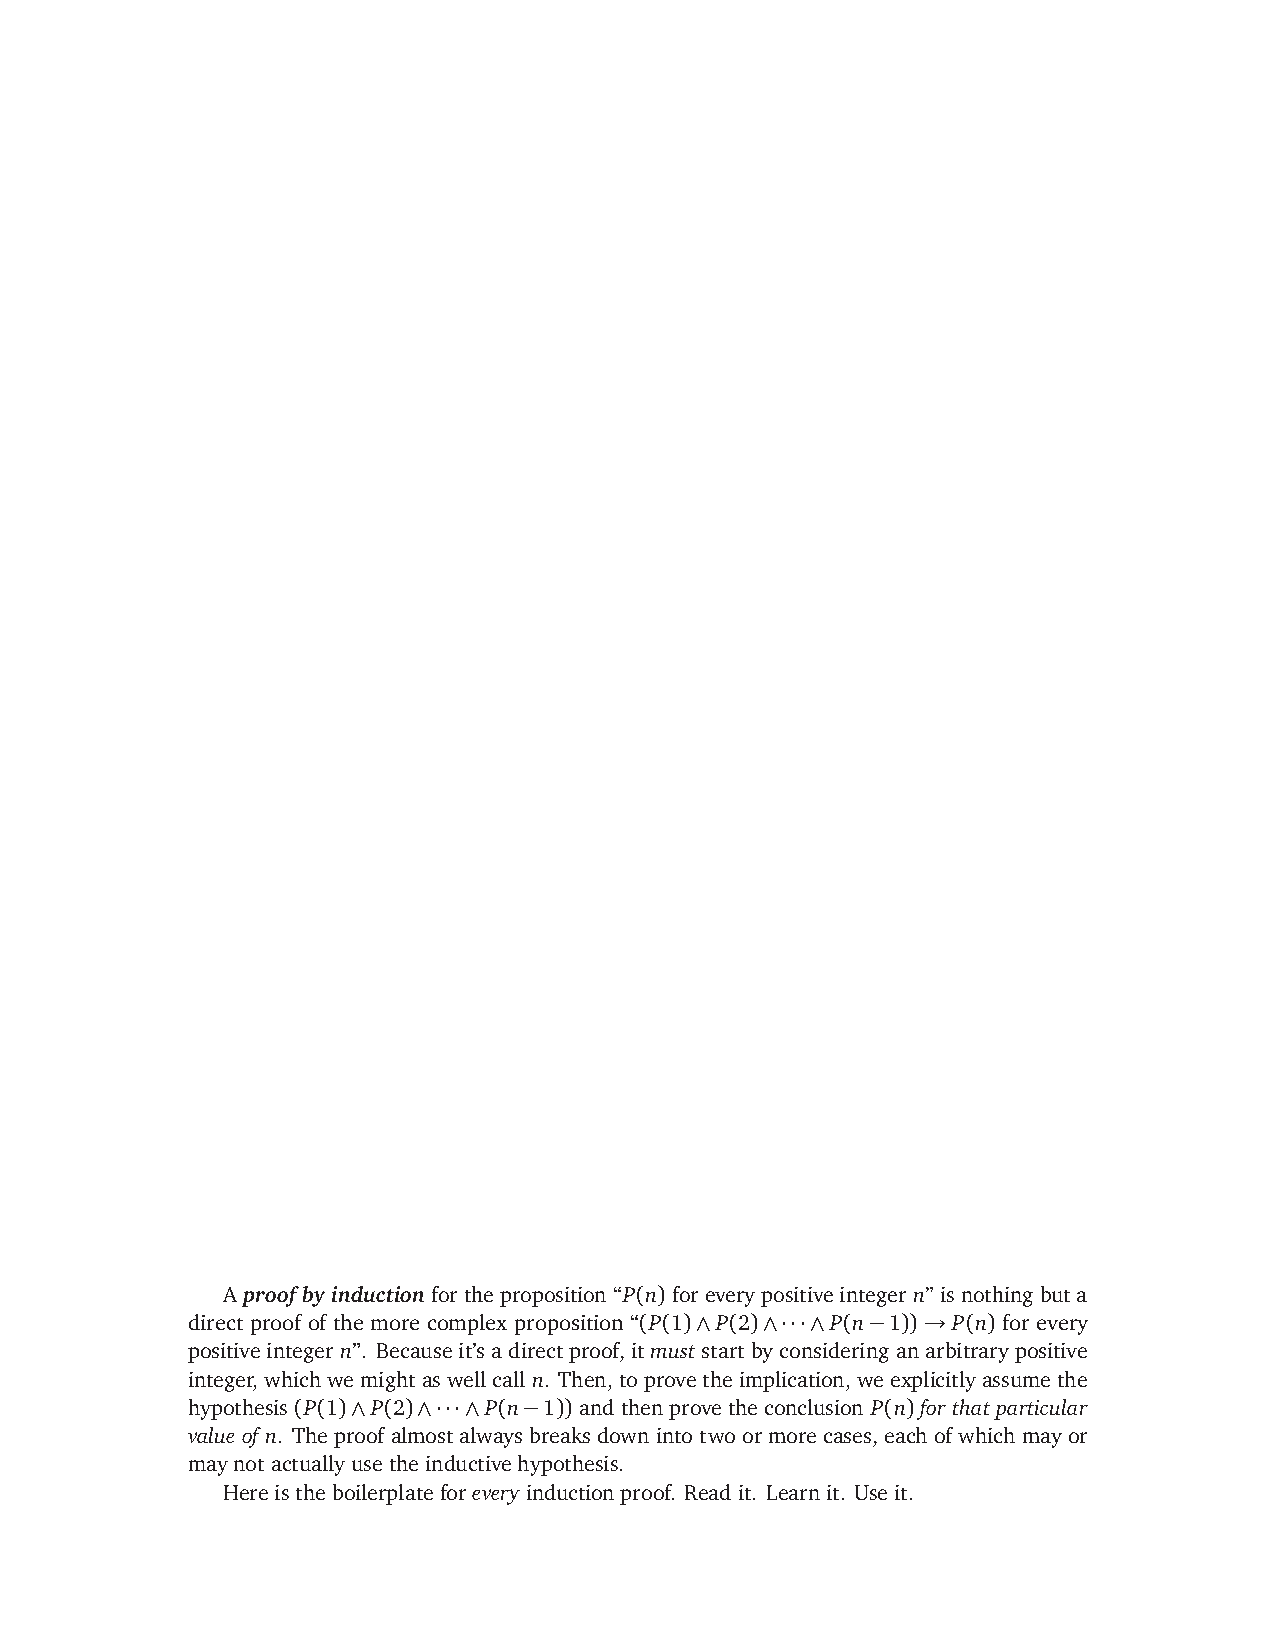
\includegraphics{w01-inductionA.pdf}\\
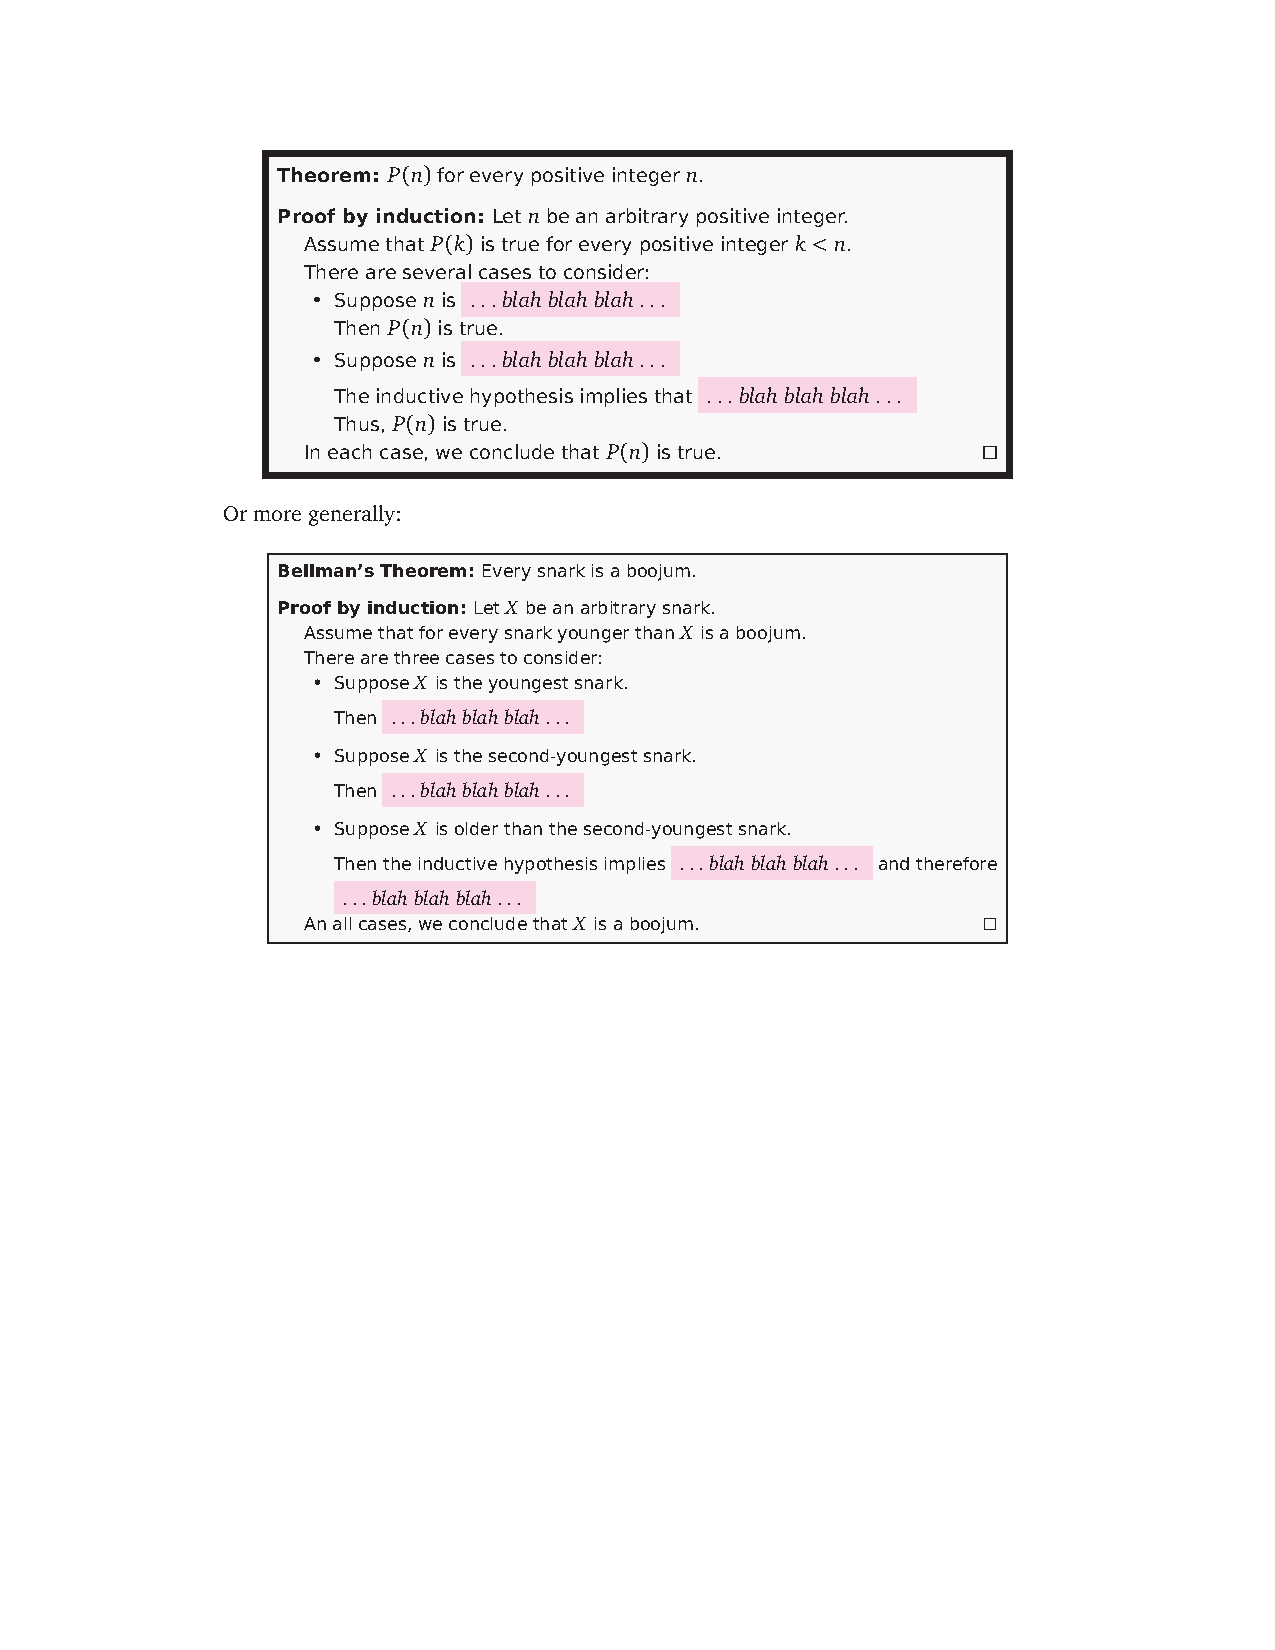
\includegraphics{w01-inductionB.pdf}

\clearpage
\subsection{Tiling the courtyard}

\begin{quote}
    \footnote{From \url{https://ocw.mit.edu/courses/6-042j-mathematics-for-computer-science-fall-2010/resources/mit6_042jf10_chap03}}During the development of MIT's famous Stata Center, as costs rose further and further beyond budget, there were some radical fundraising ideas. One rumored plan was to install a big courtyard with dimensions $2^n \times 2^n$ and to have one of the central squares\footnote{In the special case $n = 0$, the whole courtyard consists of a single central square; otherwise, there are four central squares.} be occupied by a
statue of a wealthy potential donor (who we will refer to as “Bill”, for the purposes of preserving anonymity). A complication was that the building's unconventional
architect, Frank Gehry, was alleged to require that only special L-shaped tiles be used for the courtyard. It was quickly determined that a courtyard meeting these constraints exists, at least for n = 2. But what about for larger values of n? Is there a way to tile a $2^n \times 2^n$ courtyard with L-shaped tiles around a statue in the center?
\end{quote}

\begin{theorem}
    For all $n \geq 0$ there exists a tiling of a $2^n \times 2^n$ courtyard with Bill in a central square.
\end{theorem}

Try it.

~\\\emptybox{5em}

\begin{quote}
    ``If you can't prove something, try to prove something grander!''
\end{quote}
Try again...

\vfill

\begin{quote}
    "Sometimes finding just the right induction hypothesis requires trial, error, and insight."
\end{quote}


\clearpage
\subsection{Making Change}

\begin{quote}
The country Inductia, whose unit of currency is the Strong, has coins worth 3 Sg (3 Strongs) and 5 Sg. Although the Inductians have some trouble making small change like 4Sg or 7Sg, it turns out that they can collect coins to make change for any number that is at least 8 Strongs.
\end{quote}

\begin{theorem}
    The Inductians can make change for any amount of at least 8Sg.
\end{theorem}


\clearpage
\section{Invariants}

\begin{quote}
    \footnote{From \url{https://ocw.mit.edu/courses/6-042j-mathematics-for-computer-science-fall-2010/resources/mit6_042jf10_chap03}}One of the most important uses of induction in computer science involves proving that a program or process preserves one or more desirable properties as it proceeds.
A property that is preserved through a series of operations or steps is known as an invariant. Examples of desirable invariants include properties such as a variable never exceeding a certain value, the altitude of a plane never dropping below 1,000
feet without the wingflaps and landing gear being deployed, and the temperature of a nuclear reactor never exceeding the threshold for a meltdown.

We typically use induction to prove that a proposition is an invariant. In particular, we show that the proposition is true at the beginning (this is the base case) and that if it is true after t steps have been taken, it will also be true after step t + 1 (this is the inductive step). We can then use the induction principle to conclude that  proposition is indeed an invariant, namely, that it will always hold.
\end{quote}

\subsection{The Diagonally-Moving Robot}

Suppose that you have a robot that can walk across diagonals on an infinite 2-dimensional grid. The robot starts at position (0, 0) and at each step it moves up or down by 1 unit vertically and left or right by 1 unit horizontally. To be clear, the robot must move by exactly 1 unit in each dimension during each step, since it can only traverse diagonals.

\begin{itemize}
    \item Can the robot ever reach position (1, 0)?
    \item Formulate a predicate that expresses the property that the robot can only reach positions $(x, y)$ for which
            $x + y$ is even. (Hint: Index it over the number of steps.)
    \item Prove:
\end{itemize}

\begin{theorem}
    The sum of the robot's coordinates is always even.
\end{theorem}


\clearpage
\subsection{8-puzzle}

\begin{theorem}
    No sequence of legal moves\footnote{Page 18, \url{https://ocw.mit.edu/courses/6-042j-mathematics-for-computer-science-fall-2010/resources/mit6_042jf10_chap03}} transforms the sliding board below on the left into the board below on the right.\\~

    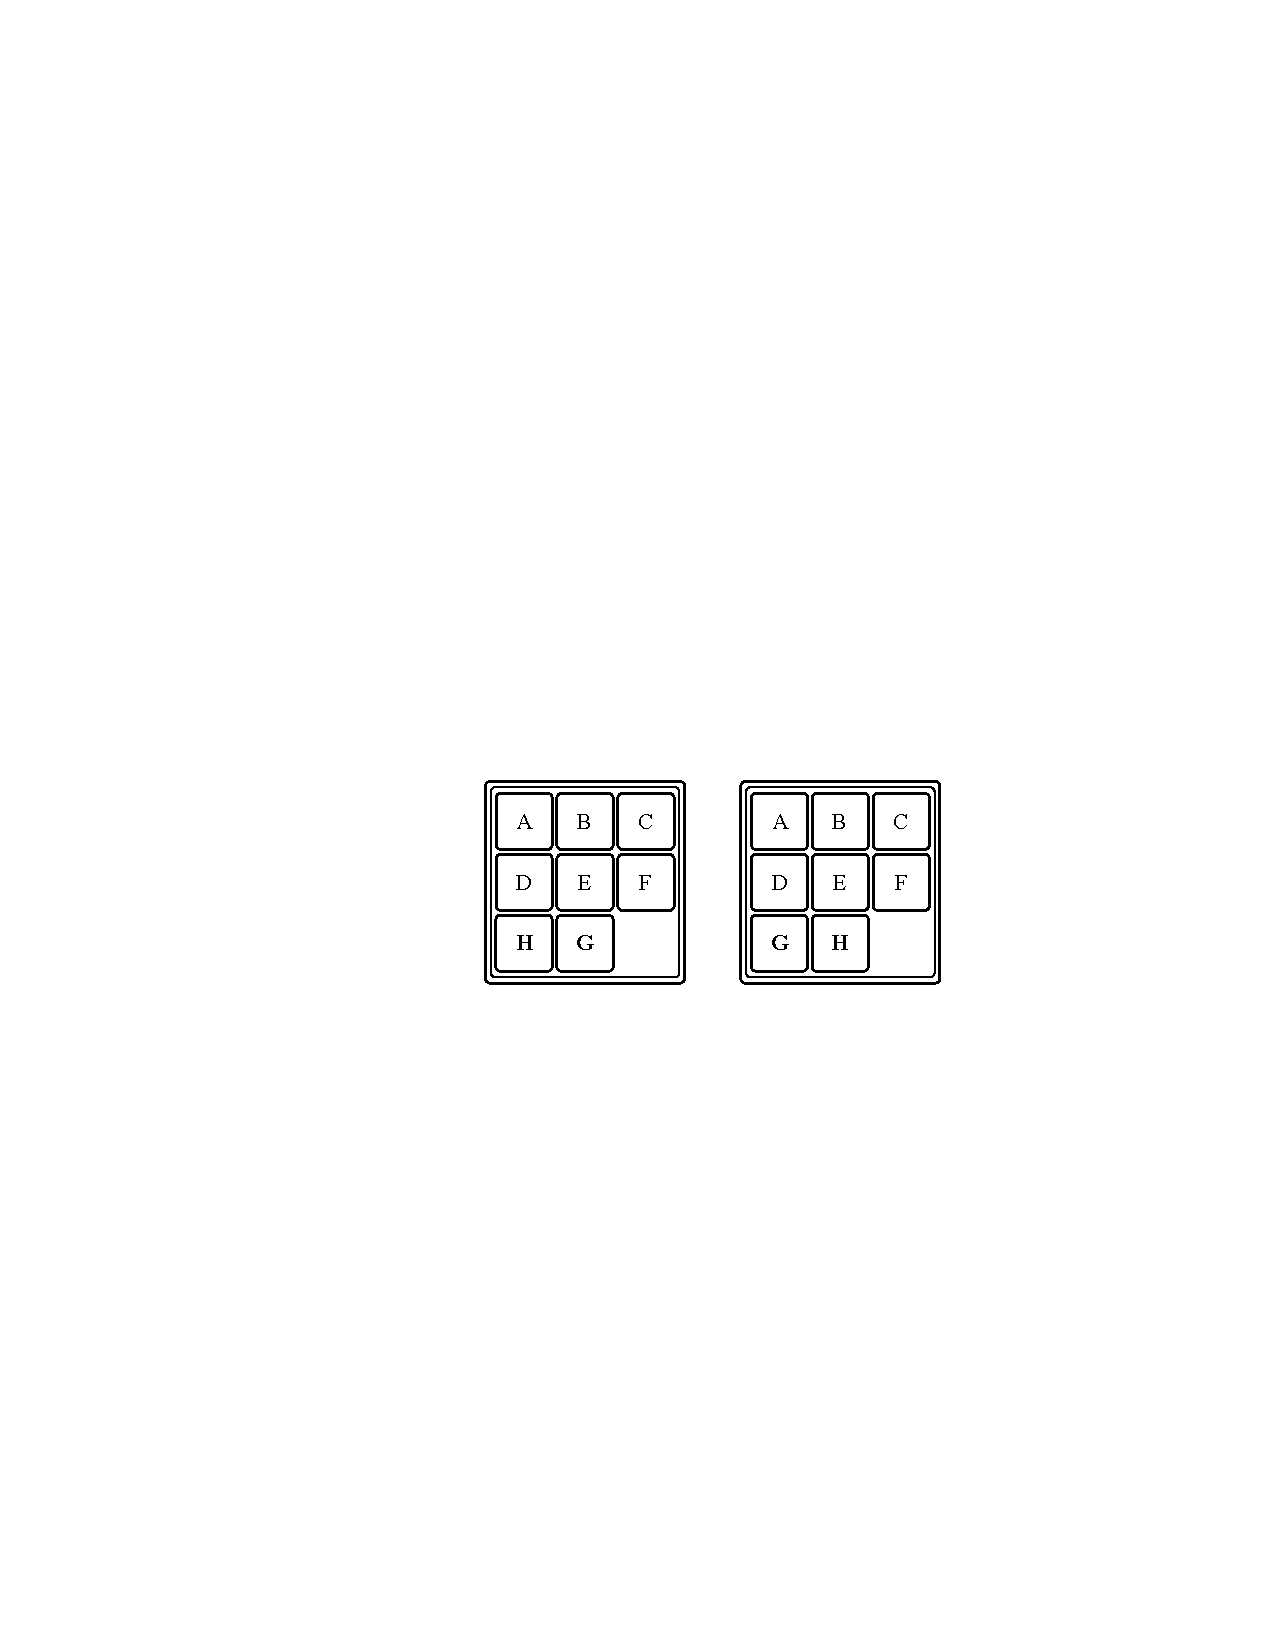
\includegraphics{w01-8puzzle.pdf}
\end{theorem}


\end{document}  